\section{Media Management S3 Component}
\label{sec:S3_component}

In this section will be analyzed the Media Management S3 Component, developed to store images and documents on cloud through Amazon S3 Service.
This specific component has been developed in order to store and manage media files in Amazon S3 service.
Operations that can be done, like upload, delete or get media, is ruled by CORS (\ref{subsec:S3_cors}) pattern.
These operations are direct: none of them is done via server. Server is only used to get the authorization to communicate with the S3 cloud storage service.
In fact, client makes an AJAX request to server in order to get the Signed URL, that is the request URL combined with the name of S3 Bucket and the dedicated Region. 
Once the client receive the Signed URL can pass the operation to S3 Service and carry it out.
Bucket and Region names are stored in \texttt{.env} file and must be set up on S3 website.

\begin {figure}[h]
\graphicspath{{images/chapter_s3/}}
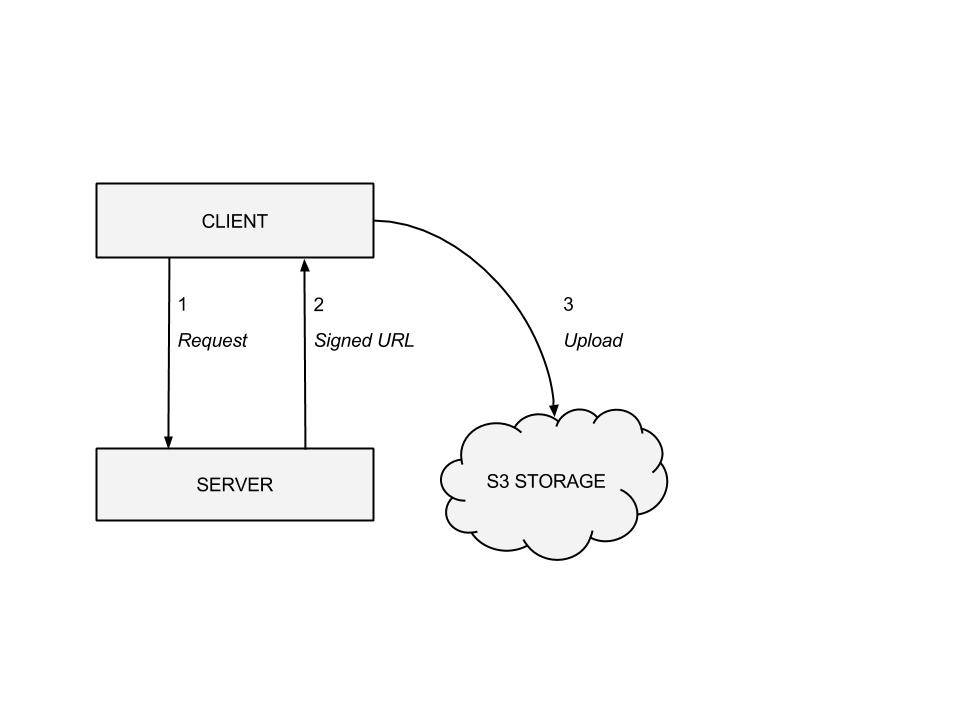
\includegraphics[width=\textwidth]{s3_upload}
\caption{S3 direct upload process}
\end {figure}



\subsection{S3 Component X-Elements}
\label{subsec:S3_server_elem}

In order to use Media Management S3 Component in an X-Project App there's need to combinate five different X-Elements, for the server-side: \texttt{api-s3-upload}, \texttt{api-s3-list}, \texttt{api-s3-delete}, \texttt{part-s3-list} and \texttt{part-s3-upload}.
Each element provides the opportunity to use one of the basic function of Amazon S3 service. 

\subsubsection{\texttt{api-s3-upload}}
\label{api-s3-upload}
The element named \texttt{api-s3-upload} needs to upload new files 

\subsubsection{\texttt{api-s3-list}}
\label{api-s3-list}
The element named \texttt{api-s3-list} makes...

\subsubsection{\texttt{api-s3-delete}}
\label{api-s3-delete}
The element named \texttt{api-s3-delete} makes...

\subsubsection{\texttt{part-s3-list}}
\label{part-s3-list}
The element named \texttt{part-s3-list} makes...

\subsubsection{\texttt{part-s3-upload}}
\label{part-s3-upload}
The element named \texttt{part-s3-upload} makes...



